\documentclass[11pt]{article}
% Online appendix to the JMLR submission; separate file, not part of the manuscript.
\usepackage{jmlr2e}
\usepackage{amsmath}
\usepackage{booktabs,multirow,subcaption}
\usepackage{microtype}
\setlength{\emergencystretch}{5em}
\usepackage{needspace}
\hypersetup{hidelinks}
\graphicspath{{figures/}{../../results/figures/}}
\usepackage{xr}
\externaldocument{main}
\newcommand{\E}{\mathbb{E}}
\newcommand{\R}{\mathbb{R}}
\newcommand{\spar}{\textsc{spar}}
\newenvironment{restated}[1]{%
  \par\medskip\noindent\textbf{#1 (restated).}\hspace{0.4em}\ignorespaces
}{\par\smallskip}

\begin{document}
\title{Online Appendix: Finite-Cadence Refresh Equilibria for Streaming Prior-Anchored Ridge}
\author{\name Mrigank Shekhar Singh \email mrigank.codes@gmail.com \\
        \addr DLDAV Model School, Shalimar Bagh\\
        Delhi, India}
\editor{}
\maketitle

\section{Extended Experimental Protocol}
\label{app:protocol}


\subsection{Factorial Grid}
\emph{Definition.}
The grid of Section~\ref{sec:experiments} is generated by \texttt{scripts/synthetic\_factorial.py}.
The main suite is the full factorial
\[
  \underbrace{\{\text{iso},\ \text{decay3},\ \text{rankdef}\}}_{\text{spectra}}
  \times
  \underbrace{\{\text{abrupt},\ \text{covrot},\ \text{both}\}}_{\text{drift}}
  \times
  \underbrace{\{\text{oracle},\ \text{warm},\ \text{adversarial}\}}_{\text{prior}}
\]
with Gaussian noise, giving 27 configurations, plus an extra suite of four: loss of persistent excitation on the decay3 spectrum, oscillating drift on the isotropic spectrum, a stationary control (no drift), and a covariance-rotation configuration with heavy-tailed $t_3$ noise, for 31 configurations in total.
Spectra: isotropic ($\mu_i \equiv 1$), decay3 (log-spaced from $1$ to $10^{-3}$, condition number $10^3$), and rank-deficient (a fixed fraction of zero eigenvalues).
Drifts: an abrupt jump of the target, a rotation of the input covariance, both combined, none, the death of excitation in a subspace, and an oscillating target.
Priors: oracle (the pre-drift target), warm (a perturbed warm-up solution), and adversarial (a perturbation independent of the target).
All configurations use $D = 128$, $T = 10^4$ steps with a warm-up of $T_w = 2000$, noise variance $\sigma^2 = 0.01$, and 5 seeds per configuration; every method runs predict-then-update.

\begin{figure}[htbp]
\centering
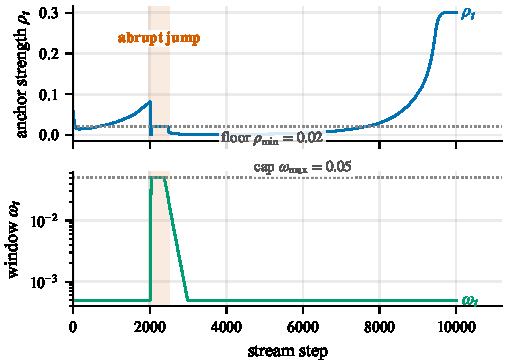
\includegraphics[width=0.55\textwidth]{F4_two_dials}
\caption{Both estimators self-calibrate on a stream with an abrupt jump ($D = 128$, decay-3, seed 0): the anchor strength $\rho_t$ falls on conflict (Proposition~\ref{prop:conflict}) and the window $\omega_t$ opens on drift (Theorem~\ref{thm:window}), both recovering; dotted lines mark the $\rho$ floor and the $\omega$ cap.}
\label{fig:cliffdials}
\end{figure}

\begin{table}[htbp]
\centering
\small
\caption{Stress suite (4 configurations $\times$ 5 seeds): mean and worst overall MSE, one fixed setting per method. The suite is deliberately outside the main grid's operating envelope (loss of persistent excitation, oscillating drift, a stationary control, heavy-tailed rotation noise); the true-noise Kalman is an oracle comparator, and the covariance-form recursion diverges in all 20 runs.}
\label{tab:stress}
\begin{tabular}{lcc}
\toprule
method & mean MSE & worst MSE \\
\midrule
Kalman, true noise ($q = 10^{-4}$) & $1.29$ & $6.26$ \\
SPAR-EG$^+$ & $1.60$ & $7.83$ \\
SPAR-EG & $1.60$ & $7.77$ \\
leaky RLS, information form ($\lambda = 0.99$) & $1.61$ & $7.70$ \\
SPAR-Pull & $1.66$ & $8.10$ \\
SGD ($\mathrm{lr} = 0.01$) & $2.07$ & $10.03$ \\
Adam ($\mathrm{lr} = 0.01$) & $2.82$ & $13.32$ \\
WiSE-FT ($\alpha = 1$) & $3.62$ & $17.39$ \\
anchor-free solve & $4.08$ & $19.70$ \\
frozen warm solution & $5.91$ & $28.83$ \\
leaky RLS, covariance form ($\lambda = 0.99$) & \multicolumn{2}{c}{diverged (20/20)} \\
\bottomrule
\end{tabular}
\end{table}

On the stress suite SPAR-EG$^+$ is the best oracle-free method in mean MSE ($1.60$), $23\%$ below SGD and $43\%$ below Adam; the true-noise Kalman leads it by $23\%$, consistent with the suite residing outside the self-calibration's design envelope (short streams and stationary controls favor fixed shrinkage, Section~\ref{sec:limitations}).

\begin{table}[htbp]
\centering
\scriptsize
\setlength{\tabcolsep}{3pt}
\caption{Marginal mean MSE over the 27 main configurations (each row averages 9 configurations $\times$ 5 seeds), addressing the aggregate-only view of Table~\ref{tab:grid}. The two SPAR methods agree within $0.03$ on every slice; the Kalman and VFF leaders are prior-independent and lose the covariance-rotation slice. The \texttt{abrupt} and \texttt{both} rows coincide to three decimals because both streams carry the same abrupt target jump, and the added covariance rotation shifts the drift-axis mean by less than $10^{-3}$.}
\label{tab:marginal}
\begin{tabular}{llccccc}
\toprule
axis & value & SPAR-Pull & SPAR-EG$^+$ & KF-slow & VFF & leaky-info \\
\midrule
spectrum & isotropic & $0.673$ & $0.644$ & $0.507$ & $0.562$ & $0.636$ \\
 & decay-3 & $0.114$ & $0.115$ & $0.065$ & $0.120$ & $0.257$ \\
 & rank-deficient & $0.131$ & $0.132$ & $0.071$ & $0.119$ & $0.134$ \\
\midrule
drift & abrupt & $0.454$ & $0.440$ & $0.310$ & $0.387$ & $0.487$ \\
 & covariance rotation & $0.011$ & $0.011$ & $0.023$ & $0.027$ & $0.054$ \\
 & both & $0.454$ & $0.440$ & $0.310$ & $0.387$ & $0.487$ \\
\midrule
prior & oracle & $0.301$ & $0.294$ & $0.215$ & $0.267$ & $0.342$ \\
 & warm & $0.305$ & $0.295$ & $0.215$ & $0.267$ & $0.342$ \\
 & adversarial & $0.313$ & $0.303$ & $0.215$ & $0.267$ & $0.342$ \\
\bottomrule
\end{tabular}
\end{table}

\emph{Methods.}
Each configuration runs the baseline families below in a common streaming protocol, plus the slow-horizon estimated-$R$ Kalman, the variable forgetting factor baselines, the two OGD variants (scalar segment and $D$-dimensional profile), SPAR-EG$^+$, and the causally-tuned Kalman filters appended post hoc. The families are the frozen warm solution, an anchor-free solve, leaky RLS at $\lambda \in \{0.999, 0.997, 0.995, 0.99\}$ in both the covariance-form recursion and the batch information-form solve, directional forgetting at the matched grid $\lambda_f \in \{0.999, 0.997, 0.995, 0.99, 0.98, 0.95, 0.90\}$, AROW at $r \in \{0.01, 0.05, 0.1, 0.3, 0.5\}$, random-walk Kalman filters at $q \in \{10^{-6}, 10^{-5}, 10^{-4}\}$ with the true noise level plus the estimated-$R$ variants at both horizons, SGD at $\mathrm{lr} \in \{0.003, 0.01\}$ and Adam at $\mathrm{lr} \in \{0.0003, 0.001, 0.003, 0.01\}$, variable forgetting factor RLS at two floors under both the single-step and the nominal-length calibrations, and the WiSE-FT $\alpha$-envelope (11 values). The SPAR methods are scalar, diagonal, two-estimator, and expert-simplex.
Sweeps are reported per value; the table reports each family's best setting under both the per-configuration rule (oracle-tuned baselines, the conservative treatment) and the global single-setting rule, and SPAR methods use the same configuration in every cell.

\emph{Baseline verification.}
Before any comparison, the \texttt{verify} step of the pipeline checks the implementation identities numerically: directional forgetting at $\lambda_f = 1$ coincides with RLS, the Kalman filter at $q = 0, R = 1$ coincides with RLS, and the WiSE-FT endpoints coincide with the frozen and fully adapted solves (maximum absolute deviation of order $10^{-15}$).
The same step checks the algebraic identities of Section~\ref{sec:theory} symbolically (sympy), and the step exits nonzero on any failure.

\emph{Estimated-noise Kalman.}
The grid includes two estimated-$R$ Kalman filters.
The fast variant updates $R$ with a 100-step moving average of squared residuals; a fast horizon attributes part of the drift-induced residual to measurement noise, which suppresses the filter's gain precisely when adaptation is needed, and it collapses to $1.09/5.36$.
The slow variant uses a $20{,}000$-step horizon (matching the SPAR noise baseline) and attains $0.215/0.93$ (best single $q = 10^{-4}$), within $5.4\%$ of the true-noise filter ($0.204/0.86$) and ahead of SPAR-Pull overall ($0.306/1.22$), though SPAR-Pull leads it on all nine covariance-rotation configurations ($0.011$ vs.\ $0.023$ per configuration mean).
Together, the two rows show that the apparent gap was caused by the estimation horizon, not by access to the true noise level.

\emph{Rank-deficiency note.}
The prediction-unit estimator never forms $\mathrm{tr}(\bar A^{-1})$: $d_{\mathrm{act}}$ counts only the eigenvalues of $\bar A$ above the $10^{-8}$ numerical ridge, so dead directions contribute neither variance nor conflict and feature rescaling leaves $\rho$ invariant (Appendix~\ref{app:hyper}).
The floor/cap pair bounds the resulting strength in all $135$ main-grid and $20$ stress-suite runs; no SPAR method diverged on any spectrum.

\emph{Divergence boundary.}
The leaky covariance-form recursion is one tuning step from failure on this grid: $\lambda = 0.997$ attains $0.555$ mean MSE, $\lambda = 0.995$ attains $182$ (worst $3{,}878$), and $\lambda = 0.99$ attains $1.2 \times 10^6$, diverging in $135/135$ main-grid and $20/20$ stress-suite runs (nominal window $100 < D = 128$); Figure~\ref{fig:cliffapp} plots the sweep.
The batch information-form solve of the same objective is stable at every $\lambda$ ($0.34$ mean at $\lambda = 0.99$), which locates the explosion in the covariance recursion rather than the objective; the family's $\lambda$-sensitivity remains (its best stable window is $1.1\times$ SPAR's).

\begin{figure}[htbp]
\centering
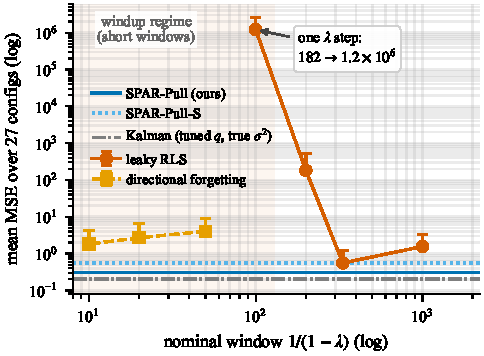
\includegraphics[width=3.1in]{F3_lambda_cliff}
\caption{Mean MSE over 27 configurations versus nominal window $1/(1-\lambda)$ (log--log; $+1$ s.d.\ whiskers). Leaky RLS degrades in one $\lambda$ step ($182 \to 1.2 \times 10^6$ at window $200 \to 100$); shading marks the windup regime ($\mathrm{window} < D = 128$); directional forgetting is divergence-free but $3.3\times$ worse at its best; SPAR-Pull and the scalar SPAR method use one fixed configuration everywhere.}
\label{fig:cliffapp}
\end{figure}
A diagnostic log of the forgetting factor (\texttt{diagnostics.py} \texttt{--diag vff}, \texttt{results/vff\_diag.csv}) confirms the degeneracy: under the reference calibration $\xi = \sigma_0^2$ the factor remains pinned at its floor on $96\%$ of steps on both stationary and drifting streams (mean $\lambda = 0.990$ at floor $0.99$), and a recursive-scale variant of the rule (a Fortescue-style running $\xi$) still pins at the floor ($92\%$ of steps, overall MSE within $2\%$ of the best fixed-$\lambda$ method).
Residual-driven forgetting degenerates to fixed-$\lambda$ leaky RLS whenever $\xi$ tracks the residual scale, a saturation documented in the variable-forgetting-factor literature \citep{paleologu2008}.
The covariance-form VFF inherits the same calibration sensitivity: the single-step normalization $\xi = \sigma_0^2$ drives the factor below $D$ and it diverges identically, while the nominal-length normalization $\xi = N_0\sigma_0^2$ of the original formulation keeps the nominal window near $N_0$ and is stable (best single setting $N_0 = 100$: $0.267/0.98$; the single-step calibration diverges in all 135 runs), the horizon choice $N_0$ playing the role of the fixed window that SPAR's window estimator sets online.
The first-order family terminates at its own boundary: at $\mathrm{lr} = 0.02$, one grid step above the swept maximum, SGD diverges on 45 of 135 runs, and at $\mathrm{lr} = 0.05$ the recursion overflows outright (\texttt{diagnostics.py} \texttt{--diag sgd}); the reported grid $\{0.003, 0.01\}$ sits at the stable frontier of the constant-step family.

\subsection{Windup Mechanism}
The covariance-form divergence obeys one law with two channels: whatever the rank-one downdate cannot see inflates by $(1{-}\omega)^{-1}$ per step, growth like $e^{\omega T}$ in the stream length.
On full-rank spectra the unseen component is roundoff: the exponentially weighted covariance matrix is a positive combination of $T \gg D$ outer products, full-rank almost surely at every window, with limiting spectral support bounded away from zero (the lower edge obeys $\lambda - \ln\lambda = 1 + c$, positive for all $c$); the iterated inverse $P \leftarrow (P - kk^\top)/(1{-}\omega)$ instead accumulates antisymmetric roundoff error, and a one-line symmetrization $P \leftarrow \tfrac12(P + P^\top)$ isolates this channel (\texttt{diagnostics.py} \texttt{--diag windup}; 2 representative configurations $\times$ 2 seeds per row):

\begin{table}[h]
\centering
\small
\caption{Mean MSE of the covariance-form leaky recursion on full-rank spectra, with and without per-step symmetrization of the iterated inverse.
At the longest window both variants agree to machine precision; at short windows the unsymmetrized recursion diverges at both dimensions while the symmetrized variant remains stable at every window tested.}
\label{tab:windup-mech}
\begin{tabular}{lccc}
\toprule
$\lambda$ ($1/(1-\lambda)$) & $D$ & standard recursion & symmetrized \\
\midrule
$0.997$ ($333$) & 128 & $1.15$ & $1.15$ \\
$0.995$ ($200$) & 128 & $25.1$ & $0.80$ \\
$0.99$ ($100$) & 128 & $2.8 \times 10^{4}$ & $0.61$ \\
$0.99$ ($100$) & 512 & $7.0 \times 10^{4}$ & $10.4$ \\
\bottomrule
\end{tabular}
\end{table}

On rank-deficient spectra the second channel is deterministic: the dead directions receive no data, so nothing downdates the corresponding block of $P$ and it inflates by $(1{-}\omega)^{-t}$ in exact arithmetic, symmetrized or not.
The appended symmetrized grid method confirms the split (\texttt{append\_arms.py}, \texttt{rls\_sym} rows of \texttt{results/factorial\_extras.csv}): stable on all 90 full-rank runs ($0.13$ mean on the ill-conditioned spectrum, $0.60$ isotropic, at $\lambda = 0.99$) and divergent on 42 of 45 rank-deficient runs ($45$ of $45$ at $\lambda = 0.97$).
The anchored information form is immune to both channels by construction---it never iterates an inverse---and Proposition~\ref{prop:windup} bounds its conditioning for any data and any window.
The single-step VFF calibration enters the same regime through its floor (windows $20$--$100$ at $\lambda_{\min} \in \{0.95, 0.99\}$); the nominal-length calibration keeps windows near $N_0$, above the amplification threshold at every setting tested.

\subsection{False-escalation Calibration}
The calibration experiment of Proposition~\ref{prop:falsealarm} runs 300 stationary streams per spectrum through the SPAR estimator with a fixed, calibrated model, records the two-scale residual statistic $z_t = (\widehat\sigma^2_{\mathrm{fast}} - \widehat\sigma^2_{\mathrm{slow}})/\sigma^2$, and measures the fraction of streams whose maximum exceeds the sliding-EMA threshold $\tau(\delta) = \sqrt{2\nu_z^2\log(T/\delta)/m_{\mathrm{eff}}}$ with $m_{\mathrm{eff}} = (2-\eta_f)/\eta_f$ at the fast gain $\eta_f = 1/h_f$ and the Gaussian excess proxy $\nu_z^2 = 2$.
The measured rate is $0.003$ on isotropic spectra at nominal $\delta = 0.10$ and $0.040$ on ill-conditioned spectra at nominal $\delta = 0.05$, at or below the nominal level; at $\delta = 0.01$ the ill-conditioned rate is $0.033$---the exceedance is predicted by the sub-exponential threshold's linear branch: at $\delta = 0.01$ and $m = 100$, the linear term $2 b_z \log(T/\delta)/(cm)$ dominates the quadratic branch, so the Gaussian-form threshold $\sqrt{2\log(T/\delta)/m}$ used in the calibration experiment is provably too low by the $b_z$-scaling of the moving-average's heavy tail, and the measured $0.033$ exceeds the nominal $0.01$ accordingly.

\subsection{Ablation and Sensitivity}
The ablation (\texttt{scripts/revision\_runs.py --suite ablation}) runs the prediction-unit method and its ablations on 4 representative configurations (abrupt and oscillating drifts, adversarial prior, ill-conditioned spectrum) $\times$ 5 seeds.
Removing the window estimator (fixed $\omega$) costs $+189\%$ overall MSE, removing the two-scale residual detector $+190\%$, and removing the pull-identity refresh $+189\%$; setting $\gamma = 0.5$ costs $+560\%$, which measures the $\gamma = 1$ principle of Appendix~\ref{app:proof-dominance}.
Freezing the strength estimator to its warm-up value \emph{lowers} overall MSE by $2.2\%$ on these configurations, and removing the variance-floor subtraction costs $+1.7\%$ under the nominal cap, with the undebiased estimator pinning the window at its cap as Theorem~\ref{thm:window} predicts.
The three-way dissociation in Table~\ref{tab:ablation} localizes the prior-immunity mechanism: freezing the spectral anchor refresh costs $2.2\times$ on the warm-prior configurations and $7.4\times$ on the adversarial ones (adversarial early MSE $47.0$ vs.\ $16.4$), whereas freezing $\rho$ leaves both within $2.6\%$.
Prior immunity is therefore carried by the refresh, and the strength estimator's role is the drift-onset conflict response measured in Appendix Figure~\ref{fig:cliffdials}---it matters only when the warm-up prior scale is unknown, where it guards against an oversized anchor.
An alternating-trust diagnostic probes the strength estimator's average-case value directly (\texttt{diagnostics.py} \texttt{--diag alt\_trust}: the target switches every 500 steps between a noisy revisit of the anchor and a drifted target, two spectra, 5 seeds): the adaptive rule attains $6.79$ overall MSE against $6.64$--$7.00$ for pinned strengths spanning three orders of magnitude ($10^{-3}$ to $1$)---a $\pm 3\%$ spread, because the anchor \emph{refresh}, not the strength estimator, carries the phase-to-phase adaptation.

\begin{table}[h]
\centering
\footnotesize
\caption{Component dissociation on the 4-configuration ablation suite (mean $\pm$ s.d.\ over 20 runs per cell; early MSE is the first 500 post-jump steps). Freezing the anchor refresh is the only variant that loses prior immunity; freezing the strength estimator is indistinguishable from the full method.}
\label{tab:ablation}
\begin{tabular}{lccc}
\toprule
variant & warm overall & adversarial overall & adversarial early \\
\midrule
full & $2.26 \pm 3.28$ & $1.04 \pm 0.21$ & $16.4 \pm 3.3$ \\
fixed $\rho$ (refresh on) & $2.20 \pm 3.16$ & $1.05 \pm 0.21$ & $16.5 \pm 3.3$ \\
frozen anchor (no refresh) & $4.98 \pm 6.49$ & $7.69 \pm 1.62$ & $47.0 \pm 10.2$ \\
no variance floor & $2.30 \pm 3.33$ & $1.06 \pm 0.21$ & $16.7 \pm 3.3$ \\
\bottomrule
\end{tabular}
\end{table}

The dichotomy is exact: the naive estimator $\hat\nu^2_{\mathrm{naive}}(\omega) = (\widehat\E[r_t^2] - \hat\sigma^2)\omega^2$ yields a cubed estimator $(T_{\mathrm{naive}}(\omega))^3 = (\omega^*)^3 + 4\omega^3/(2-\omega) > 2\omega^3$ for every $\omega \in (0,2)$, so the cubed trajectory doubles each iteration and reaches the cap in $O(\log)$ steps even at zero drift (\texttt{naive\_dial\_no\_fixed\_point}), while the variance-floor-subtracted estimator gives the exact affine contraction $u_{m+1} = (1-\eta_\nu)u_m + \eta_\nu(\omega^*)^3 \to (\omega^*)^3$ from any initialization (\texttt{debiased\_dial\_contraction})---both formalized in \texttt{Core.lean}.
Replacing $\mathrm{tr}(\bar A^{-1})$ with the ridge-damped trace $\mathrm{tr}((\bar A + \rho I)^{-1})$ on the rank-deficient configurations (\texttt{append\_damped\_trace.py}, \texttt{results/damped\_trace.csv}) yields identical error ($0.100$ vs.\ $0.100$ overall): the residual-detector and floor branches govern the estimator where the trace saturates, and the damped variant is the numerically preferred implementation on ill-conditioned spectra.
The sensitivity variants (legacy parameter-unit method, \texttt{results/ablation\_spar\_kf.csv}; the control constants are shared with the prediction-unit method) scale the residual horizons ($\pm$), the refresh cadence ($10 \to 50$), the reference-anchor cadence, and the window cap ($0.05 \to 0.02$ and $0.10$): six of the seven variants change overall MSE by at most $\pm 10\%$, and the largest change is the window cap $\omega_{\max} = 0.02$ at $+16\%$.

\subsection{The Conflict Estimator at Drift Onset}
\label{app:transient}

Table~\ref{tab:transient} pins the strength at $\rho \in \{0.01, 0.1, 1\}$ with the refresh on and compares it with the adaptive estimator on the abrupt-jump stream with the decay-3 spectrum (5 seeds; \texttt{scripts/transient\_test.py}, \texttt{results/transient\_test.csv}).
At cadence $k = 10$ the adaptive estimator is $1\%$ below the best fixed strength and the large-anchor policy costs $87\%$ more; at $k = 50$ it is within $5\%$ of the best fixed strength while the large-anchor policy costs $2.8\times$.
The penalty is pre-drift, not post-jump: $\rho = 1$ multiplies the pre-drift MSE by $4.2$ relative to the small fixed anchor ($0.049$ vs.\ $0.012$ at $k = 10$) because the anchor holds a warm prior that the decaying spectrum no longer supports, whereas the $50$-step post-jump window is dominated by the jump magnitude and is flat across the adaptive and small-anchor policies---if anything slightly better for the large anchor ($7.7$ vs.\ $9.5$).
On the isotropic spectrum, where a scalar strength has no structural effect, every policy has the same pre-drift MSE ($0.0104$) and differs only through the post-jump term.
We therefore read $\rho_t$ as a guard against a badly oversized anchor---the failure mode a good warm prior invites---not as a post-jump accelerator.

\begin{table}[!htbp]
\centering
\footnotesize
\caption{Transient strength sweep on the abrupt-jump stream, decay-3 spectrum, 5 seeds: pre-drift MSE, MSE over the $50$ steps after the jump, and overall MSE.
The refresh is on in every row; the adaptive row is the paper's method and the others pin $\rho$ for the whole stream.}
\label{tab:transient}
\begin{tabular}{ccccc}
\toprule
$k$ & strength policy & pre-drift MSE & post-jump MSE $[0,50]$ & overall MSE \\
\midrule
10 & adaptive & $0.0136$ & $9.48$ & $\mathbf{0.166}$ \\
10 & fixed $\rho = 0.01$ & $0.0116$ & $9.48$ & $0.168$ \\
10 & fixed $\rho = 0.1$ & $0.0271$ & $9.49$ & $0.195$ \\
10 & fixed $\rho = 1$ & $0.0489$ & $7.72$ & $0.311$ \\
\midrule
50 & adaptive & $0.0197$ & $9.52$ & $0.254$ \\
50 & fixed $\rho = 0.01$ & $0.0146$ & $9.54$ & $\mathbf{0.243}$ \\
50 & fixed $\rho = 0.1$ & $0.0338$ & $9.56$ & $0.308$ \\
50 & fixed $\rho = 1$ & $0.0495$ & $8.52$ & $0.723$ \\
\bottomrule
\end{tabular}
\end{table}

\subsection{Coupling Verification}
Theorem~\ref{thm:closedloop}(i)'s condition is measured directly (\texttt{diagnostics.py} \texttt{--diag coupling}, \texttt{results/coupling\_diag.csv}): on the four ablation configurations $\times$ 5 seeds, each estimator is pinned at $\pm 10\%$ of its converged value while the other adapts, and the two sensitivities $L_{\omega\rho}$ (of the cubed window target) and $L_{\rho\omega}$ (of the strength target) are finite-differenced at the empirical coupled fixed point.
The product $L_{\omega\rho} L_{\rho\omega} < 1$ holds in 20 of 20 runs, with maximum $5.7 \times 10^{-3}$---$174$ to $1381$ times below one on the oscillating configuration, the only one with both estimators interior.
On three of the four configurations one estimator saturates at its cap or floor, making the corresponding sensitivity exactly zero---a pinned estimator realizes the triangular specialization of Theorem~\ref{thm:closedloop}(ii), and the large cubed-coordinate slopes recorded at floored windows are boundary artifacts of perturbing a microscopic $u = \omega^3$, multiplied by an exactly-zero factor: the caps act as the coupling control, and the cross-signs at the interior fixed point match the theory ($u^*$ increasing in $\rho$, $\rho^*$ decreasing in $u$).

\subsection{Spectral-risk Verification}
Theorem~\ref{thm:rmt}(i)'s closed form was validated at three levels (\texttt{diagnostics.py} \texttt{--diag rmt}).
First, at $45$ fixed operating points (three spectra, including a rank-deficient one, $\times$ five nominal windows $1/(1-\lambda) \in \{100, \dots, 2000\}$ $\times$ three anchor strengths $\rho \in \{10^{-3}, 10^{-2}, 10^{-1}\}$), the formula matches direct Monte Carlo simulation of the anchored solve ($40$ stationary streams per point, oracle anchor) within $4.4\%$ relative error across the entire range, including aspect ratios $\zeta = D\omega$ above one and the rank-deficient spectrum, whose active directions the formula restricts to exactly (\texttt{results/rmt\_grid.csv} records the grid, \texttt{results/rmt\_rankdef.csv} the active-subspace invariance, and \texttt{results/rmt\_verify.csv} the method-level checks).
Second, at the method's own operating points---the converged estimator pairs $(\omega, \rho)$ measured on stationary streams per spectrum---the formula predicts the method's stationary pre-drift MSE within $1.9\%$ (rank-deficient), $12.7\%$ (ill-conditioned), and $9.8\%$ (isotropic, where the strength estimator sits at its cap), with no fitted parameter.
Third, the closed-form sensitivities of part~(ii) agree with numerical differentiation of the fixed point to $10^{-6}$ relative error.
The pre-drift MSE reported in Section~\ref{sec:experiments} ($1.01$--$1.14 \times \sigma^2$ across spectra) is the segment average including the post-warm-up transient; the formula describes the stationary value at the converged operating pair.

\subsection{Per-step Cost}
Table~\ref{tab:app-ops} reports the per-step wall-clock cost of the closed-form methods at $D = 2048$ (fp64 CPU, \texttt{scripts/bench\_ops.py}; run alone for clean timing).
The cached-basis per-direction head is $O(D^2)$ per step with $O(D^3)$ at refreshes; the scalar method solves the anchored system exactly at $O(D^3)$ per step, and its spectral refresh reuses the solve's factorization in $O(D^2)$ (Section~\ref{sec:method-solve}).
The information form deliberately trades the covariance recursion's $O(D^2)$ rank-one update for a factorization that does not wind up on rank-deficient spectra (Proposition~\ref{prop:windup}); where per-step cost dominates, the cached-basis head is the intended path.

\begin{table}[h]
\centering
\footnotesize
\caption{Per-step cost at $D = 2048$ (fp64 CPU).
The cached-basis per-direction head projects each feature into the last refresh's eigenbasis and solves the diagonal system ($O(D^2)$/step, $O(D^3)$ every $k$ refreshes); the scalar method performs a Cholesky factorization plus triangular solves per step ($O(D^3)$), which motivates the per-direction path at large $D$.}
\label{tab:app-ops}
\begin{tabular}{lc}
\toprule
method & ms/step at $D = 2048$ \\
\midrule
leaky RLS & $32.0$ \\
AROW & $31.3$ \\
Kalman & $53.0$ \\
directional forgetting & $56.3$ \\
SPAR-Pull-D (cached basis, $O(D^2)$/step) & $52.6$ \\
SPAR-Pull-S (exact scalar solve, $O(D^3)$/step) & $241$ \\
\bottomrule
\end{tabular}
\end{table}
SPAR-EG and SPAR-EG$^+$ run four batch solves per step (the frozen anchor is the remaining expert in the pool), so their per-step cost is about four times the scalar SPAR-Pull solve timed here; the cached-basis path applies to them as well.

\subsection{Mismatched Generators}

\begin{figure}[h]
\centering
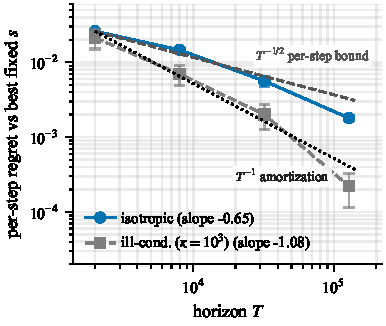
\includegraphics[width=2.9in]{F7_regret_scaling}
\caption{Average per-step regret of the segment (scalar-pull) OGD method versus horizon $T$ (log--log; whiskers: $\pm 1$ s.d.\ over 5 seeds; the drift phase lasts a fixed $1{,}000$ steps at every horizon).
Fitted slopes $-0.65$ (isotropic) and $-1.08$ (ill-conditioned, $\kappa = 10^3$) lie inside the $T^{-1/2}$ per-step rate (dashed) implied by the scalar $O(\sqrt T)$ Zinkevich bound (the $D = 1$ member of the Proposition~\ref{prop:ocowrap}(i) family, formalized as \texttt{ogd\_regret\_segment} in \texttt{Ogd.lean}), with the $T^{-1}$ amortization limit (dotted) as the mechanical floor.}
\label{fig:regret}
\end{figure}

At a fixed horizon, the dimension sweep separates the two gradient variants.
With $T = 9{,}000$, the drift phase held at $1{,}000$ steps, $D \in \{8, 32, 128\}$, and 5 seeds (\texttt{scripts/regret\_dscaling.py}, \texttt{results/regret\_dscaling.csv}), both methods' per-step regret is measured against the best fixed scalar pull (an 11-point segment grid, each comparator method carrying its own refresh trajectory).
The profile method's regret exceeds the segment method's at every operating point, and the gap widens monotonically with $D$---from $0.001$ to $0.078$ on isotropic spectra and from $3 \times 10^{-6}$ to $0.011$ on ill-conditioned spectra---the empirical signature of the $\sqrt{D}$ dimension factor in the Proposition~\ref{prop:ocowrap}(i) bound; on the full grid the same premium appears as the profile method's higher mean MSE ($0.707$ vs.\ $0.585$, Table~\ref{tab:grid}).

\begin{figure}[h]
\centering
\begin{subfigure}[t]{0.48\textwidth}
\centering
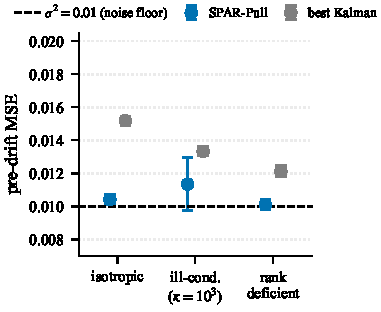
\includegraphics[width=2.55in]{F5_noise_floor}
\caption{}
\label{fig:floor}
\end{subfigure}\hfill
\begin{subfigure}[t]{0.48\textwidth}
\centering
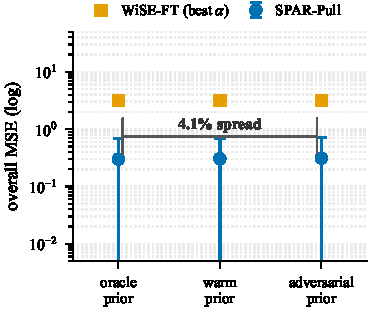
\includegraphics[width=2.55in]{F6_prior_immunity}
\caption{}
\label{fig:prior}
\end{subfigure}
\caption{(a) Pre-drift MSE remains at the irreducible floor $\sigma^2 = 0.01$ across all three spectra (dots show 5-seed means $\pm 1$ s.d.\ against the best tuned-$q$ Kalman with true $\sigma^2$), illustrating Proposition~\ref{prop:conflict} at the optimum.
(b) Overall MSE (log scale) across oracle, warm, and adversarial priors (means over all runs).
While the WiSE-FT best-$\alpha$ envelope sits near $3.2$ under every prior, SPAR-Pull varies by only $4.1\%$ across all three priors (bracket): Proposition~\ref{prop:minimax}.}
\label{fig:floorprior}
\end{figure}

Three generators violate the linear-Gaussian, constant-rate model class: nonlinear targets ($y = \tanh(x^\top w^*) + \varepsilon$; the linear head is misspecified), covariate shift (the feature scale doubles mid-stream), and a noise-regime change ($\sigma^2$ rising from $0.01$ to $0.05$ at $t_1$, with no target drift).
On nonlinear targets (four configurations: decay3 and isotropic spectra under abrupt, gradual, and stationary drifts; 5 seeds each) SPAR-EG$^+$ attains $0.221$ overall MSE, SPAR-EG $0.222$, the best single leaky window ($\lambda = 0.997$) $0.232$, and SPAR-Pull $0.273$: the mixture shifts weight toward the expert that tolerates the nonlinearity.
Under covariate shift the Kalman family leads ($0.268$ with the true noise, $0.284$ with the slow estimated $R$), while SPAR-EG$^+$ and SPAR-Pull lead the anchored and leaky methods ($0.490$ and $0.492$), ahead of the batch-solved leaky method ($0.550$), SPAR-EG ($0.566$), and the best single leaky window ($0.627$), the two-scale residual detector catching the scale change.
Under the noise-regime change (two configurations, decay3 and isotropic spectra, 5 seeds each) the fast-horizon estimated-$R$ Kalman attains $0.069$--$0.098$, its $20{,}000$-step-horizon sibling $0.084$--$0.110$, and the true-noise filter $0.096$--$0.114$ (its fixed $R$ is wrong after the change), while the SPAR-EG mixture attains $0.047$--$0.087$ and SPAR-EG$^+$ $0.047$--$0.053$; SPAR-Pull holds $0.052$ on the decay3 spectrum but lags at $0.080$ on the isotropic spectrum, where its slow noise baseline tracks the pre-change level.
No SPAR method diverged under any mismatch, while the $\lambda = 0.995$ leaky method diverged on nonlinear targets (two of five seeds on the decay3 spectrum under abrupt drift) and degraded under the noise change ($9.1$ and $9.4\times 10^3$ overall MSE).

\subsection{A Real High-dimensional Stream: Hourly Electricity Load}
\label{app:realstream}

The factorial grid is synthetic, so we also run the grid-default configuration, unchanged, on a real stream: the public hourly electricity-load panel (321 clients, $26{,}304$ hours) \citep{trindade2015electricity,lai2018lstd}.
Features at hour $t$ are the standardized log-loads of all 321 clients plus an intercept and hour-of-day sine/cosine ($D = 324$); the target is the log-load of one held-out client (the 25th-percentile client by mean load) one hour ahead, centered on its warm-up mean.
The warm-up is $2{,}000$ hours and the evaluation horizon $6{,}000$ hours, so $T > 5{,}000$ and $D > 128$ as required.
The stream is not stationary: load carries daily and weekly cycles and a seasonal trend, and the target series moves with them.

Both SPAR methods use the grid defaults of Table~\ref{tab:hyper} unchanged: window range $[5 \times 10^{-4}, 0.05]$, refresh cadence 10, residual horizon 30, and the drift-active floor $0.02$.
The baselines are swept on the same stream and reported at their best setting, which is oracle tuning in their favour: leaky RLS over $\lambda \in \{0.99, 0.995, 0.999\}$ and the slow estimated-$R$ Kalman over $q \in \{10^{-4}, 10^{-5}\}$.

\begin{table}[!htbp]
\centering
\footnotesize
\setlength{\tabcolsep}{5pt}
\caption{Real stream (hourly electricity load, $D = 324$, $T = 6{,}000$ evaluation hours, 25th-percentile held-out client): MSE of the next-hour log-load over the full horizon and over the final $2{,}000$ hours.
SPAR methods use the factorial-grid defaults with no stream-specific tuning; baseline hyperparameters are swept on the same stream and reported at their best.}
\label{tab:electricity}
\begin{tabular}{lcc}
\toprule
method & full horizon & final $2{,}000$ h \\
\midrule
leaky RLS, information form ($\lambda = 0.999$) & $\mathbf{0.0209}$ & $\mathbf{0.0134}$ \\
leaky RLS ($\lambda = 0.995$) & $0.0219$ & $0.0160$ \\
leaky RLS ($\lambda = 0.99$) & $0.0228$ & $0.0174$ \\
Kalman, slow estimated $R$ ($q = 10^{-5}$) & $0.0660$ & $0.0170$ \\
Kalman, slow estimated $R$ ($q = 10^{-4}$) & $0.3054$ & $0.0183$ \\
\midrule
SPAR-EG$^+$ (grid defaults) & $0.0212$ & $0.0143$ \\
SPAR-Pull (grid defaults) & $0.0232$ & $0.0154$ \\
\bottomrule
\end{tabular}
\end{table}

\begin{table}[!htbp]
\centering
\footnotesize
\setlength{\tabcolsep}{5pt}
\caption{Real stream, held-out client sweep: MSE of the next-hour log-load over the full $6{,}000$-hour horizon for the 25th-, 50th-, and 75th-percentile clients by mean load.
The oracle column is the best of the three leaky windows ($\lambda \in \{0.99, 0.995, 0.999\}$) chosen \emph{per client} ($\lambda = 0.999, 0.995, 0.995$ at the 25th, 50th, 75th percentiles)---tuning in the baseline's favour---while the SPAR methods use the grid defaults with no stream-specific tuning.
Bold marks the best entry in each row.}
\label{tab:electricity-clients}
\begin{tabular}{lccc}
\toprule
held-out client & best oracle leaky & SPAR-EG$^+$ & SPAR-Pull \\
\midrule
25th percentile & $\mathbf{0.0209}$ & $0.0212$ & $0.0232$ \\
50th percentile & $0.0086$ & $\mathbf{0.0083}$ & $0.0090$ \\
75th percentile & $\mathbf{0.0112}$ & $0.0113$ & $0.0130$ \\
\midrule
three-client mean & $\mathbf{0.0136}$ & $\mathbf{0.0136}$ & $0.0151$ \\
\bottomrule
\end{tabular}
\end{table}

Across the sweep, SPAR-EG$^+$ lands within $1.2\%$ of the per-client oracle window and $4.3\%$ below it at the 50th percentile, and it matches the oracle on the three-client mean ($0.0136$ both); SPAR-Pull is $4.2$--$16.5\%$ above the oracle.
The ordering of the closed-form methods is stable across the three clients, so the untuned transfer is not specific to a single reported percentile.

Three observations.
First, the untuned SPAR-EG$^+$ lands $1.1\%$ above the best oracle-tuned leaky window over the full horizon and $6.3\%$ above it on the final $2{,}000$ hours, while SPAR-Pull is $10.7\%$ and $14.7\%$ above; a smooth seasonal stream has a long and nearly constant optimal window, which is exactly the regime in which a fixed long window is close to optimal and adaptation has little to recover.
Second, the slow estimated-$R$ Kalman is far worse over the full horizon ($0.051$ and $0.257$) and still $26\%$ above the leaky baseline on the final $2{,}000$ hours, i.e.\ its early noise estimates are poor and it only recovers late.
Third, no method diverges and the ordering of the closed-form methods is stable across the horizon, so the control law transfers to a real $D = 324$ stream without retuning.

\section{BCI IV Details}
\label{app:eeg}


\emph{Datasets and protocol.}
BCI Competition IV 2a \citep{brunner2008bci2a} and 2b \citep{leeb2008bci2b}, nine subjects each, loaded from the npz cache described in Appendix~\ref{app:repro}.
Cross-session protocol: each method fits on the training session and streams the evaluation session (288 trials on 2a, 320 on 2b) predict-then-update.
All online methods use supervised adaptation: the label of trial $t$ enters after its prediction, so every prediction is prequential.
Labels are one-hot $Y_t \in \{0,1\}^K$; the streaming head maintains a $D \times K$ coefficient matrix and the scalar residual driving both estimators is $r_t^2 = \|Y_t - \widehat Y_t\|_2^2/K$.
The metric is balanced accuracy; with $n = 9$ subjects per data set we report paired tests and effect sizes, not significance alone.

\begin{table}[h]
\centering
\scriptsize
\setlength{\tabcolsep}{2.5pt}
\renewcommand{\arraystretch}{0.86}
\caption{BCI IV cross-session, balanced accuracy (mean $\pm$ s.d.\ over 9 subjects per data set).
Supervised online protocol for adaptive methods; classical methods are static. $^{\mathrm{T}}$Session-level Euclidean alignment from the unlabeled evaluation session (transductive); the online-EA row is strictly causal.
Highest value per column in bold.}
\label{tab:eeg}
\begin{tabular}{lcc}
\toprule
method & BCI IV 2a & BCI IV 2b \\
\midrule
\multicolumn{3}{l}{\emph{classical (canonical implementations)}}\\
MDM (pyriemann) & $0.566 \pm 0.160$ & $0.728 \pm 0.148$ \\
FgMDM (pyriemann) & $0.641 \pm 0.171$ & $0.755 \pm 0.149$ \\
LDA (raw features) & $0.480 \pm 0.069$ & $0.651 \pm 0.107$ \\
LDA (raw) + session EA$^{\mathrm{T}}$ & $0.563 \pm 0.076$ & $0.677 \pm 0.133$ \\
CSP-LDA (mne) & $0.607 \pm 0.151$ & $0.749 \pm 0.141$ \\
tangent cov + LDA & $0.637 \pm 0.165$ & $0.752 \pm 0.147$ \\
cov-LDA, offline session-EA$^{\mathrm{T}}$ & $0.664 \pm 0.173$ & $0.728 \pm 0.159$ \\
\midrule
\multicolumn{3}{l}{\emph{ours (closed-form streaming, predict-then-update)}}\\
CSP + SPAR-Pull & $0.627 \pm 0.159$ & $0.770 \pm 0.142$ \\
tangent cov + SPAR-Pull & $0.527 \pm 0.151$ & $0.772 \pm 0.129$ \\
hybrid + SPAR-Pull$^{\mathrm{T}}$ & $0.597 \pm 0.137$ & $0.808 \pm 0.104$ \\
hybrid + SPAR-Pull, grid defaults$^{\mathrm{T}}$ & $0.579 \pm 0.137$ & $0.801 \pm 0.101$ \\
online-EA + hybrid + SPAR-Pull & $0.596 \pm 0.134$ & $0.801 \pm 0.105$ \\
hybrid + AAL head ($\gamma{=}1$, fixed anchoring)$^{\mathrm{T}}$ & $0.608 \pm 0.139$ & $0.799 \pm 0.107$ \\
hybrid + leaky head$^{\mathrm{T}}$ & $0.554 \pm 0.123$ & $0.812 \pm 0.108$ \\
hybrid + SPAR-EG$^{\mathrm{T}}$ & $0.580 \pm 0.130$ & $\mathbf{0.816 \pm 0.102}$ \\
hybrid + SPAR-EG$^{+\,{\mathrm{T}}}$ & $0.586 \pm 0.141$ & $0.813 \pm 0.107$ \\
\midrule
\multicolumn{3}{l}{\emph{backprop references}}\\
EEGNet-lite (train-split tuned, zero-shot) & $0.556 \pm 0.080$ & $0.776 \pm 0.129$ \\
WiSE-FT on the net (causal, $\alpha$-envelope) & $0.591 \pm 0.079$ & $0.811 \pm 0.115$ \\
\midrule
post-hoc ensemble (cov-LDA + hybrid warm fit)$^{\mathrm{T}}$ & $\mathbf{0.668 \pm 0.175}$ & $0.771 \pm 0.104$ \\
\bottomrule
\end{tabular}
\end{table}

\emph{Compute.}
The complete closed-form suite (feature extraction plus all closed-form methods) for all nine 2b subjects runs in $17$ s on the CPU used here ($1.9$ s per subject; \texttt{results/tier1\_rerun\_2b.log}); one EEGNet-lite training configuration ($120$ epochs) trains on the WSL GPU environment, and the full backprop protocol trains three configurations per subject plus the online fine-tuning pass.

\emph{Feature families.}
Three feature families feed the readouts of Table~\ref{tab:eeg}.
CSP: 6-component CSP (Ledoit--Wolf shrinkage, log output) computed with MNE \citep{gramfort2013mne} on bandpassed epochs (8--30 Hz, 4th-order Butterworth), the classical motor-imagery standard \citep{ramoser2000csp}.
Tangent covariance: per-trial log-Euclidean covariance tangent features (lower triangle) on bandpassed epochs, the feature family of pyriemann's tangent-space methods.
Hybrid: the statistical pipeline (summary statistics, lags $(1, 2, 4, 8)$, FFT bins) concatenated with the tangent-covariance features.
Classical readouts are MDM and FgMDM as implemented in pyriemann \citep{barachant2020pyriemann}, raw-feature LDA with and without session-level Euclidean alignment \citep{he2020ea}, CSP-LDA, tangent-covariance LDA (shrinkage LDA in all cases), and a covariance-LDA method with the same offline alignment.
Streaming readouts are the two-estimator SPAR-Pull head (anchor refresh every 5 trials), the AAL head (fixed $\gamma = 1$ anchoring), and a forgetting-only leaky head, each applied to CSP, tangent-covariance, or hybrid features.

\emph{Alignment protocol.}
The hybrid methods use session-level Euclidean alignment: per-trial covariance whiteners are computed from each session separately, so the alignment is transductive at the session level (the offline classical methods share this convention).
The strictly online method recomputes its whitener causally from a trailing window of the evaluation stream (40 trials, refreshed every 10) for \emph{both} feature halves: the statistical features and the tangent-covariance features are each whitened with the trailing-window estimate, so no stream feature depends on trials beyond the current one.
All SPAR methods in Table~\ref{tab:eeg} run the same variance-floor-subtracted window inversion as the factorial grid (Theorem~\ref{thm:window}), with the estimator ranges rescaled to the $288$-trial stream (window range $[5\times10^{-3},0.02]$, refresh cadence 5, residual horizon 40, calibration blocks 2).
The \emph{grid defaults} row is the same hybrid head with the factorial-grid window range, refresh cadence, residual horizon, and calibration blocks ($[5\times10^{-4},0.05]$, 10, 30, 10); the gap to the EEG-range row prices those four settings ($0.018$ balanced accuracy on 2a and $0.007$ on 2b).
The reduced range therefore helps, but the ranking of the readouts and the qualitative conclusion (closed-form streaming matches the causal backprop reference) do not depend on it.

\emph{WiSE-FT protocol measurement.}
Transplanting the original WiSE-FT protocol \citep{wortsman2022wiseft} (fine-tune on the target data, then evaluate on it) into cross-session evaluation is train-on-test.
Measured directly, the offline fine-tuned endpoint reaches accuracy $1.000$ by memorizing the evaluation stream.
The comparison we report is therefore the causal reformulation: the network is fine-tuned online with one SGD step per trial \emph{after} predicting it, trial $t$ is predicted with the interpolation $(1 - \alpha)\,W_{\mathrm{zero}} + \alpha\,W_t$ where $W_t$ is the online model before trial $t$'s label, and the $\alpha$-envelope is swept post-hoc over 11 values with all trajectories causal (the prequential evaluation of Table~\ref{tab:eeg}).

\emph{Backprop references.}
EEGNet-lite is a small EEGNet variant \citep{lawhern2018eegnet} ($F_1 = 8$, $D = 2$, $F_2 = 16$) trained with Adam.
Its hyperparameters (epochs, learning rate) are selected on an 80/20 split of the training session from the grid $(120, 10^{-3})$, $(300, 10^{-3})$, or $(300, 3 \times 10^{-4})$ with no evaluation-session access, then retrained on the full training session and evaluated zero-shot on the evaluation session.
The WiSE-FT-on-network reference uses this zero-shot model as its frozen endpoint and the causal fine-tuning protocol above.

\section{Hyperparameters and Provenance}
\label{app:hyper}


\emph{Fixed constants and the default control parametrization.}
The complete fixed control parametrization is enumerated in Table~\ref{tab:hyper}: the three headline constants (anchor-refresh cadence 10 steps, fast-EMA residual horizon 30 steps, drift-active anchor-strength floor $\rho \ge 0.02$), the clip ranges of both estimators, the slow-noise-EMA baseline horizon (20{,}000, matched to the estimated-noise Kalman), the reference-anchor EMA horizon (200 steps), the conflict-floor multiplier ($\tfrac12$), the estimator smoothing gains ($\eta_C = 0.15$, $\eta_\nu = 0.2$), and the $10^{-8}$ numerical ridge of the trace and active-dimension computations.
These were fixed once, before the factorial grid, and are shared by every SPAR method on it; all remaining behavior is self-calibrated at runtime by the two online estimators.
The sensitivity analysis of Appendix~\ref{app:protocol} perturbs the headline constants directly.

\begin{table}[htbp]
\centering
\small
\caption{Fixed default control parametrization (grid: $T = 10^4$). The EEG head uses a reduced estimator range and shorter horizons for the short evaluation streams, hand-set once and disclosed here; no per-configuration search was performed for any SPAR method.}
\label{tab:hyper}
\begin{tabular}{lll}
\toprule
parameter & grid default & EEG head \\
\midrule
refresh cadence $k$ & $10$ & $5$ trials \\
fast-EMA horizon $h_f$ & $30$ & $40$ \\
warm-up anchor strength $\rho_0$ & $0.1$ & $0.1$ \\
stationary $\rho$ floor & $10^{-5}$ & $10^{-5}$ \\
drift-active $\rho$ floor & $0.02$ & --- \\
anchor-strength cap $\rho_{\max}$ & $1.0$ & $1.0$ \\
window clip $[\omega_{\min}, \omega_{\max}]$ & $[5\times10^{-4},\ 0.05]$ & $[5\times10^{-3},\ 0.02]$ \\
slow-noise-EMA horizon & $20{,}000$ & $2{,}000$ \\
reference-anchor EMA horizon & $200$ & $30$ \\
conflict-floor multiplier & $\tfrac12$ & $\tfrac12$ \\
smoothing gains $(\eta_C, \eta_\nu)$ & $(0.15,\ 0.2)$ & $(0.2,\ 0.1)$ \\
active-dimension / trace ridge & $10^{-8}$ & $10^{-8}$ \\
\bottomrule
\end{tabular}
\end{table}

\emph{Estimator floors and caps.}
The window estimator is clipped to $\omega \in [5 \times 10^{-4},\ 0.05]$ on the grid (the floor is no forgetting at the grid's horizon; the cap bounds the forgetting rate), and the anchor-strength estimator enforces the drift-active floor above together with a hard cap.
The EEG head uses a reduced range suited to the short evaluation streams ($\omega \in [5 \times 10^{-3},\ 0.02]$, fast horizon 40, refresh every 5 trials, reference-anchor horizon 30, smoothing gains $(\eta_C,\eta_\nu) = (0.2, 0.1)$) and omits the drift-active floor; these are the only stream-dependent settings in the paper.

\emph{Conflict estimator branches (prediction units).}
Algorithm~\ref{alg:spar-pull} step (iv) takes the maximum of three branches, all in prediction-risk units $[y^2]$ (the residual EMAs are $\sigma^2_{\mathrm{fast}}$ = fast EMA of $r_t^2$ at horizon $h_f$, $\sigma^2_{\mathrm{slow}}$ = slow EMA at horizon $20{,}000$; $d_{\mathrm{act}}$ is the number of eigenvalues of $\bar A$ above the $10^{-8}$ numerical ridge):
(i) the reference branch $C^\Sigma_{\mathrm{ref}} = (G_{\mathrm{ref}} - \widehat w)^\top \bar A\,(G_{\mathrm{ref}} - \widehat w) - \widehat V^\Sigma$, where $\widehat w$ is the minimum-ridge data solve, $\widehat V^\Sigma = \hat\sigma^2 d_{\mathrm{act}}/n$, and $G_{\mathrm{ref}}$ is the reference anchor (a slow-moving copy of $G$ at the reference cadence, updated every $5k$ steps);
(ii) the residual branch $C^\Sigma_{\mathrm{resid}} = E_t = \max(0, \sigma^2_{\mathrm{fast}} - \sigma^2_{\mathrm{slow}})$;
(iii) the floor $C^\Sigma_{\mathrm{floor}} = \tfrac12\,\hat\sigma^2 d_{\mathrm{act}}/T_w$ (the warm-up prediction variance is an irreducible lower bound on the conflict of a warm-up anchor).
The per-clip strength is $\rho = \mathrm{clip}(\bar\mu\,\widehat V^\Sigma/\widehat C^\Sigma_t,\ \rho_{\min}^{\mathrm{drift}},\ \rho_{\max})$ with the drift-active floor $0.02$ engaged while the window is at least half open ($\omega_t \ge \tfrac12\omega_{\max}$) and the stationary floor $10^{-5}$ otherwise.
Every branch has units $[y^2]$ and $\rho$ has units $[x^2]$; no inverse of $\bar A$ is formed, so the estimator is invariant to feature rescaling and immune to the rank-deficient trace blow-up.
The legacy parameter-unit form (with $\mathrm{tr}(\bar A^{-1})$ and $C_{\mathrm{resid}}=E_t\mathrm{tr}(\bar A^{-1})/(n\bar\mu)$) is reported only as the ablation of Appendix~\ref{app:protocol}.

\emph{Method identifiers.}
The paper's display names map to frozen artifact identifiers (internal Python/CSV keys) as follows: SPAR-Pull is \texttt{spar\_pull} (its legacy parameter-unit form is \texttt{spar\_kf2}), SPAR-Pull-S is \texttt{spar\_scalar}, SPAR-Pull-D is \texttt{spar\_diag}, SPAR-EG is \texttt{spar\_eg}, SPAR-EG$^+$ is \texttt{spar\_eg\_plus}, the causally-tuned Kalman filters are \texttt{kf\_causal} and \texttt{kf\_est\_causal}/\texttt{kf\_est\_slow\_causal}, the AAL head is \texttt{hybrid-pam\_g1}, leaky RLS is \texttt{leaky[$\lambda$]} in covariance form and \texttt{leaky\_batch} in information form, directional forgetting is \texttt{df[$\lambda_f$]}, AROW is \texttt{arow[$r$]}, the Kalman filters are \texttt{kf[$q$]} (true noise), \texttt{kf\_est} (100-step estimated $R$), and \texttt{kf\_est\_slow} (20{,}000-step estimated $R$), the gradient-descent baselines are \texttt{sgd} and \texttt{adam}, the OGD variants are \texttt{ogd\_profile} (scalar segment) and \texttt{ogd\_profile\_d} (full $D$-dimensional profile), the variable forgetting factor baseline is \texttt{vff[fortescue]} in covariance form and \texttt{vff\_info[fortescue]} in information form, and the WiSE-FT envelope is \texttt{wiseft}.
All renaming in the paper is display-layer only; the CSVs, scripts, and tests key on the artifact identifiers.

\emph{Seeds.}
All seeds are pinned in the drivers: the factorial grid uses seeds 0--4 per configuration; the ablation, regret scaling, coupling diagnostic, and mismatched-generator studies use seeds 0--4; the false-escalation calibration uses 300 streams (seeds 1000--1299); the estimator-trajectory figure uses seed 0; the EEG evaluation uses subjects 1--9 per data set (all available subjects); the BP references train with per-subject seeds equal to the subject index.
Seeds are shared across methods at each configuration.

\emph{Data manifests.}
Synthetic streams are generated from the pinned seeds by the committed generator (\texttt{rls\_baselines.make\_stream\_fac}), so no synthetic data files are needed.
The EEG evaluation reads the committed npz cache (\texttt{data/eeg\_cache/\{2a,2b\}/subject*.npz}), exported from the MNE data directory by \texttt{scripts/export\_eeg\_npz.py}.
Every result table in the paper is machine-printed from a committed CSV under \texttt{results/} (Appendix~\ref{app:repro}).

\section{Reproducibility}
\label{app:repro}


\emph{One driver.}
A single driver regenerates every figure and every wired result table from the committed caches:
\begin{quote}
\ttfamily
py scripts/run\_all.py --list\ \ list the pipeline steps\\
py scripts/run\_all.py --steps quick\ \ verify+aggregate+figures\\
py scripts/run\_all.py\ \ everything (hours; resumable)
\end{quote}
The quick preset takes about 2 minutes; the full run takes hours and is resumable.
\begin{table}[!htbp]
\centering
\footnotesize
\setlength{\tabcolsep}{4pt}
\caption{One driver, \texttt{scripts/run\_all.py}, runs these stages in order; each is resumable.}
\label{tab:pipeline}
\begin{tabular}{@{}p{0.72in}p{2.95in}p{1.55in}@{}}
\toprule
stage & driver & output \\
\midrule
\texttt{verify} & \texttt{verify\_spar\_theorems.py} & symbolic identities \\
\texttt{factorial} & \texttt{synthetic\_factorial.py} & \texttt{factorial\_d\_*.csv} \\
\texttt{sparkf} & SPAR-Pull append & \texttt{factorial\_extras.csv} \\
\texttt{append} & \texttt{append\_arms.py}, \texttt{regen\_spar\_eg\_plus.py}, \texttt{revision\_runs.py --suite grid} & \texttt{factorial\_pu\_refresh.csv} \\
\texttt{aggregate} & \texttt{aggregate\_factorial.py} & Table~\ref{tab:grid} \\
\texttt{ablation} & \texttt{revision\_runs.py --suite ablation} & \texttt{ablation\_spar\_pull.csv} \\
\texttt{falseesc} & 300-stream calibration & \texttt{false\_esc.csv} \\
\texttt{regret} & horizon and dimension scaling & \texttt{regret\_*.csv} \\
\texttt{ops} & wall-clock timing at $D=2048$ & \texttt{ops\_table.csv} \\
\texttt{eeg} & \texttt{bench\_eeg\_tier1.py} & \texttt{eeg\_tier1\_2*.csv} \\
\texttt{bp} & backprop baselines & \texttt{bp\_tta\_2*.csv} \\
\texttt{figures} & \texttt{make\_figures.py} & \texttt{results/figures/} \\
\bottomrule
\end{tabular}
\end{table}

\emph{Environment.}
Python 3.12 with the committed \texttt{requirements.txt} (jax, numpy, scipy, pandas, scikit-learn, matplotlib, sympy).
Float64 is required for the streaming solves and is enabled by setting \texttt{JAX\_ENABLE\_X64=1} (the drivers set it); a CPU runtime is recommended for the fp64 streams.
The backprop methods run on the WSL GPU virtual environment: \texttt{scripts/run\_bp\_tta\_2a.sh} and \texttt{scripts/run\_bp\_tta\_2b.sh}, with \texttt{BP\_PYTHON} pointing at that environment's interpreter and GPU extras in \texttt{requirements-wsl.txt}.

\emph{EEG data.}
Raw BCI IV files live under the MNE data directory (\texttt{MNE\_DATA} environment variable or the mne configuration; default \texttt{\~{}/mne\_data}) at the BNCI database path.
The loader prefers the npz cache: run \texttt{scripts/export\_eeg\_npz.py} once to produce \texttt{data/eeg\_cache/\{2a,2b\}/subject*.npz} for all nine subjects per data set.

\emph{Electricity data.}
The real stream of Appendix~\ref{app:realstream} reads the public hourly electricity-load panel (321 clients, $26{,}304$ rows, headerless comma-separated) from \texttt{data/ts/electricity.csv} (the loader also accepts the \texttt{.txt} variant); the file is a public download and is not shipped with the artifact.
It regenerates with \texttt{scripts/bench\_stream\_real.py --clients 11,82,171} (\texttt{results/stream\_electricity.csv}); the script accepts any client indices, and the tables report the 25th-, 50th-, and 75th-percentile clients.
The transient strength sweep of Appendix~\ref{app:transient} regenerates with \texttt{scripts/transient\_test.py} (\texttt{results/transient\_test.csv}).
The grid-default BCI row of Table~\ref{tab:eeg} is the \texttt{hybrid-spar\_kf\_grid} column of \texttt{scripts/bench\_eeg\_tier1.py}; on 2a it is also reproduced by the cheaper \texttt{scripts/eeg\_grid\_default\_probe.py}, which saves \texttt{results/eeg\_griddefault\_2a.csv}.

\emph{Lean.}
The proof artifact builds with the elan-managed Lean 4 toolchain and Mathlib via lake; the full recipe, including the Mathlib cache fetch, is \texttt{theory/lean/build\_ogd.sh} (Appendix~\ref{app:lean}).

\emph{Artifact layout.}
Every number in the paper is machine-printed into \texttt{results/*.csv} by the drivers above, and every figure is redrawn from those CSVs: the factorial tables (\texttt{factorial\_*}), the ablation (\texttt{ablation\_spar\_pull.csv}), the false-escalation calibration (\texttt{false\_esc.csv}), the regret scaling (\texttt{regret\_scaling.csv}), the cost table (\texttt{ops\_table.csv}), the EEG tables (\texttt{eeg\_tier1\_2*.csv}, \texttt{spar\_eeg\_2*.csv}, \texttt{bp\_tta\_2*.csv}), the estimator trajectory (\texttt{estimator\_trajectory.csv}), the real electricity stream (\texttt{stream\_electricity.csv}), and the transient strength sweep (\texttt{transient\_test.csv}).
The offline session-EA cov-LDA method and the post-hoc ensemble (members: the cov-LDA method and the static hybrid warm fit, identifier \texttt{ens-covlda+hybrid}) regenerate from the \texttt{eeg} step's baseline pass (\texttt{scripts/bench\_eeg.py}, recorded in \texttt{eeg\_2*.csv}); all other rows regenerate from the tier-1 pass.
The Lean material (six files, the build script, and the axiom-listing script) is under \texttt{theory/lean/}.

\bibliography{references}

\end{document}
